\documentclass[12pt,a4paper]{article}

\usepackage[utf8]{inputenc}
\usepackage[T1]{fontenc}
\usepackage[english]{babel}
\usepackage{geometry}
\usepackage{hyperref}
\usepackage{booktabs}
\usepackage{parskip}
\usepackage{microtype}
\usepackage{fancyhdr}
\usepackage{lmodern}
\usepackage{titlesec}
\usepackage{tikz}
\usetikzlibrary{arrows.meta, positioning, fit, backgrounds}

\geometry{top=2.5cm, bottom=2.5cm, left=3cm, right=3cm}

\hypersetup{colorlinks=true, linkcolor=black, urlcolor=blue}

\pagestyle{fancy}
\fancyhf{}
\rhead{Cloud Computing -- Project Draft}
\lhead{TechFix Cloud-Native Migration}
\cfoot{\thepage}

\title{
    \vspace{-1cm}
    \Large\textbf{Cloud-Native Migration of TechFix}\\[0.4em]
    \normalsize Cloud Computing Course --- Project Draft
}
\author{Filippo Palmieri \and [Partner Name]}
\date{July 2026}

\begin{document}

\maketitle
\thispagestyle{fancy}

% ============================================================
\section{The Application: TechFix}
% ============================================================

TechFix is a web application that manages post-sales technical assistance for a consumer goods company. The platform connects three types of users: technicians working at service centers across the territory, internal company staff responsible for documenting known issues, and administrators who oversee the entire system.

The core workflow is simple. When a technician encounters a product problem, they consult TechFix to find the documented malfunction and its repair solution. Staff members keep this knowledge base up to date by adding and editing malfunctions and solutions. The administrator manages users, service centers, and product assignments.

The application is built as a monolithic Laravel~10 application backed by a single MySQL database. All roles share the same codebase and run as one process on one server.

% ============================================================
\section{Challenges and Proposed Solutions}
% ============================================================

The monolithic deployment introduces several limitations. We focus on the ones most relevant to the course and describe how each is addressed.

\paragraph{Scalability.} The application has no way to handle load spikes. A realistic scenario is a product recall: many technicians simultaneously consult the catalog and malfunction pages, creating a sudden burst of read-heavy traffic. We address this with Kubernetes Horizontal Pod Autoscaling, which automatically adds more application replicas when CPU load rises and removes them when it drops.

\paragraph{Database as a bottleneck.} Under autoscaling, multiple application replicas all connect to the same MySQL instance, which becomes the bottleneck for reads. Since TechFix's workload is read-heavy (technicians read far more than staff writes), we introduce a MySQL read replica. Laravel natively supports routing reads to a replica and writes to the primary, distributing the database load without application changes.

\paragraph{Security isolation.} Currently, all components share the same machine with no network segmentation. We address this with two measures: Kubernetes Network Policies that restrict pod-to-pod traffic, and container hardening that reduces the privileges of each running process.

\paragraph{Secrets management.} Credentials are stored as plain text in a \texttt{.env} file. We store all sensitive values as Kubernetes Secrets with encryption at rest enabled, so secrets are never stored unencrypted on disk.

\paragraph{Infrastructure provisioning.} The deployment is tied to a fixed server. OpenNebula provides the virtual machines that underlie the entire stack, serving as the IaaS layer.

% ============================================================
\section{Architecture}
% ============================================================

The system is organized in two layers: OpenNebula at the bottom, providing virtual machines, and Kubernetes on top, orchestrating the application containers. Figure~\ref{fig:architecture} shows the overall layout.

\begin{figure}[h]
\centering
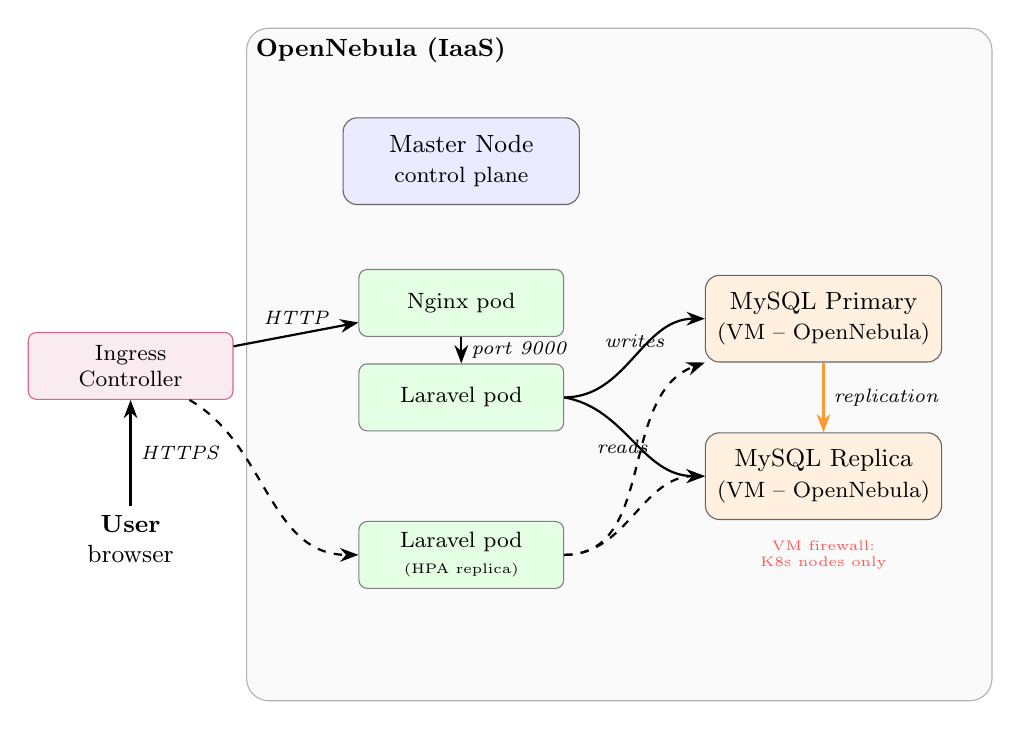
\begin{tikzpicture}[
    font=\small,
    >=Stealth,
    % Node styles
    vmbox/.style={
        rectangle, rounded corners=5pt,
        draw=black!60, fill=blue!8,
        minimum width=3cm, minimum height=1.1cm,
        align=center
    },
    dbbox/.style={
        rectangle, rounded corners=5pt,
        draw=black!60, fill=orange!12,
        minimum width=3cm, minimum height=1.1cm,
        align=center
    },
    podbox/.style={
        rectangle, rounded corners=3pt,
        draw=black!50, fill=green!10,
        minimum width=2.6cm, minimum height=0.85cm,
        align=center, font=\footnotesize
    },
    ingressbox/.style={
        rectangle, rounded corners=3pt,
        draw=purple!60, fill=purple!8,
        minimum width=2.6cm, minimum height=0.85cm,
        align=center, font=\footnotesize
    },
    workerfit/.style={
        rectangle, rounded corners=4pt,
        draw=blue!40, fill=blue!4,
        inner sep=8pt
    },
    clusterfit/.style={
        rectangle, rounded corners=6pt,
        draw=blue!50, fill=blue!2,
        inner sep=14pt
    },
    onebulafit/.style={
        rectangle, rounded corners=8pt,
        draw=gray!60, fill=gray!4,
        inner sep=18pt
    },
    lbl/.style={font=\scriptsize\itshape},
    policylbl/.style={font=\tiny, text=red!65, align=center},
]

%% ---- COLUMN 1: User + Ingress ----
\node[ingressbox]   (ingress)  at (0, 0)     {Ingress\\Controller};
\node[font=\small, align=center] (user) at (0, -2.2) {\textbf{User}\\browser};

%% ---- COLUMN 2: Worker Node 1 (Nginx + Laravel) ----
\node[podbox]  (nginx)    at (4.2,  0.8)  {Nginx pod};
\node[podbox]  (laravel1) at (4.2, -0.4)  {Laravel pod};

\begin{scope}[on background layer]
  \node[workerfit, fit=(nginx)(laravel1),
        label={[font=\footnotesize\bfseries, anchor=north]north:Worker Node 1}]
        (worker1) {};
\end{scope}

%% ---- COLUMN 2: Worker Node 2 (HPA replica) ----
\node[podbox]  (laravel2) at (4.2, -2.4)  {Laravel pod\\{\tiny (HPA replica)}};

\begin{scope}[on background layer]
  \node[workerfit, fit=(laravel2),
        label={[font=\footnotesize\bfseries, anchor=north]north:Worker Node 2}]
        (worker2) {};
\end{scope}

%% ---- COLUMN 2: Master Node ----
\node[vmbox] (master) at (4.2, 2.6) {Master Node\\{\footnotesize control plane}};

%% ---- Kubernetes cluster boundary ----
\begin{scope}[on background layer]
  \node[clusterfit, fit=(master)(worker1)(worker2),
        label={[font=\footnotesize\bfseries, text=blue!60, anchor=north west]north west:Kubernetes Cluster}]
        (k8s) {};
\end{scope}

%% ---- COLUMN 3: MySQL VMs ----
\node[dbbox] (dbprimary) at (8.8,  0.6) {MySQL Primary\\{\footnotesize (VM -- OpenNebula)}};
\node[dbbox] (dbreplica) at (8.8, -1.4) {MySQL Replica\\{\footnotesize (VM -- OpenNebula)}};

%% ---- OpenNebula outer boundary ----
\begin{scope}[on background layer]
  \node[onebulafit, fit=(k8s)(dbprimary)(dbreplica),
        label={[font=\small\bfseries, anchor=north west]north west:OpenNebula (IaaS)}]
        (onebula) {};
\end{scope}

%% ---- ARROWS ----
% User -> Ingress
\draw[->, thick] (user) -- node[right, lbl]{HTTPS} (ingress);

% Ingress -> Nginx
\draw[->, thick] (ingress) -- node[above, lbl]{HTTP} (nginx);

% Nginx -> Laravel1
\draw[->, thick] (nginx) -- node[right, lbl]{port 9000} (laravel1);

% Ingress -> Laravel2 (HPA)
\draw[->, thick, dashed] (ingress) to[out=-30, in=180] (laravel2);

% Laravel1 writes -> DB Primary
\draw[->, thick] (laravel1.east) to[out=0, in=180]
    node[above, lbl, pos=0.5]{writes} (dbprimary.west);

% Laravel1 reads -> DB Replica
\draw[->, thick] (laravel1.east) to[out=-10, in=180]
    node[below, lbl, pos=0.4]{reads} (dbreplica.west);

% Laravel2 -> DBs (dashed, same routing)
\draw[->, thick, dashed] (laravel2.east) to[out=0, in=200] (dbprimary.south west);
\draw[->, thick, dashed] (laravel2.east) to[out=0, in=180] (dbreplica.west);

% Primary -> Replica (replication)
\draw[->, thick, draw=orange!80] (dbprimary) --
    node[right, lbl]{replication} (dbreplica);

%% ---- NETWORK POLICY LABELS ----

\node[policylbl] at (8.8, -2.4) {VM firewall:\\K8s nodes only};

\end{tikzpicture}
\caption{System architecture. Solid arrows show primary traffic; dashed arrows show HPA replica traffic. MySQL runs on dedicated OpenNebula VMs outside the Kubernetes cluster.}
\label{fig:architecture}
\end{figure}

The key architectural decision is keeping MySQL outside Kubernetes. Relational databases require stable, predictable storage and write ordering that container orchestration can complicate. Running MySQL on dedicated VMs -- managed by OpenNebula -- gives us a simpler, more reliable setup. This also demonstrates a more nuanced use of OpenNebula: it is not just a host for the Kubernetes nodes, but infrastructure that serves different roles depending on the workload. The Kubernetes cluster handles stateless, scalable application logic; OpenNebula VMs handle stateful, stable database workloads.

% ============================================================
\section{Scaling Strategy}
% ============================================================

We configure Horizontal Pod Autoscaling on the Laravel deployment. Kubernetes monitors CPU utilization across the running Laravel pods. When the average exceeds a defined threshold, it automatically creates additional replicas to distribute the work; when the load drops, it removes the extra replicas. A minimum of 2 replicas ensures basic redundancy at all times.

The MySQL read replica complements the pod autoscaler: as more Laravel pods handle incoming requests, their read queries are distributed to the replica rather than all hitting the primary instance.

For the demo, we will simulate a product recall by generating concurrent HTTP requests to the catalog and malfunction endpoints and show the pod count increasing in real time.

% ============================================================
\section{Security}
% ============================================================

\paragraph{Network isolation.} We use Kubernetes Network Policies to restrict traffic between pods: the database accepts connections only from the Laravel pods, and the Laravel containers accept traffic only from Nginx. The MySQL VMs additionally have host-level firewall rules that block any connection not originating from the Kubernetes worker nodes, and block all outbound internet traffic from the database VMs. This limits lateral movement: compromising one component does not automatically grant access to others.

\paragraph{Container hardening.} All application containers run as a non-root user, with a read-only root filesystem (write access is granted only to directories that genuinely need it, such as Laravel's cache and log directories), and with Linux capabilities dropped to the minimum required. These settings are enforced through Kubernetes security contexts.

\paragraph{Secrets management.} All sensitive values (database credentials, application keys, TLS certificates) are stored as Kubernetes Secrets with encryption at rest enabled on the \texttt{etcd} datastore. This means secrets are never stored as plain text on disk, and are never embedded in container images or committed to the repository. Containers receive secrets as environment variables or mounted files at runtime.

\paragraph{TLS.} All traffic between users' browsers and the cluster is encrypted. The Ingress Controller terminates TLS and redirects plain HTTP to HTTPS. A self-signed certificate is used for the draft; the final deployment will use a proper certificate.

% ============================================================
\section{Summary of Design Choices}
% ============================================================

\begin{center}
\begin{tabular}{lll}
\toprule
\textbf{Concern} & \textbf{Choice} & \textbf{Rationale} \\
\midrule
IaaS & OpenNebula & Required; hosts all VMs \\
Orchestration & Kubernetes & PaaS layer for containers \\
App containers & Docker (multi-stage) & Small, reproducible images \\
Database & Dedicated VM (outside K8s) & Avoids StatefulSet complexity \\
DB read scaling & MySQL primary-replica & Laravel native read/write split \\
App scaling & Kubernetes HPA & Handles read-heavy load spikes \\
Network isolation & K8s NetworkPolicy + VM firewall & Defense in depth \\
Container security & SecurityContext (non-root, read-only) & Least privilege \\
Secrets & K8s Secrets + etcd encryption & No plain text on disk \\
TLS & Self-signed cert on Ingress & Traffic encryption \\
\bottomrule
\end{tabular}
\end{center}

\end{document}
